% =====================================================================
%  RESULTADOS (versión de revisión)
%  Correcciones del 4 de noviembre: ideas enlazadas, menos repeticiones y la secuencia
%  de la detención de la navegación con el apagado del portátil. Ninguna cifra de
%  resultado sale del capítulo.
% =====================================================================
\chapter{Resultados}
\label{cap:resultados}

Las dos campañas se presentan por separado porque responden a preguntas distintas. La de simulación, con treinta misiones, da la evidencia estadística sobre la tasa de éxito. La de los agentes físicos, con diez misiones sorteadas en los pisos 3 y 4 del edificio Catalayud, muestra que el sistema completo se puede llevar a un edificio real, donde intervienen los sensores, la red inalámbrica y la tracción de los agentes, y donde los usuarios piden, siguen y confirman las misiones desde un teléfono. En las dos campañas, todos los fallos ocurrieron en la navegación de un agente, sobre todo en la precisión de su llegada, y ninguno en la asignación ni en el relevo, que son el núcleo del proyecto.

% ---------------------------------------------------------------------
\section{Evaluación en simulación}
\label{sec:res-sim}

En la campaña se ejecutaron treinta misiones sorteadas (anexo A, video 6): quince con origen y destino en el mismo piso, sin relevo, que sirven de comparación, y quince entre pisos, con un relevo. Según el programa de análisis la campaña es válida, sin ningún descarte, frente a un máximo admitido del 20~\%.

\subsection{Tasa de éxito}

Una misión es exitosa si la pose final queda a 0,25~m o menos del destino, medida contra la odometría, sin importar lo que informe Nav2, y si llega a completarse sin pasar por fallo. La tabla~\ref{tab:exito} da la tasa de cada grupo con su intervalo de confianza de Wilson al 95~\% \autocite{wilson1927probable}.

\begin{table}[htbp]
  \caption{Tasa de éxito de la campaña en simulación, con intervalo de confianza
    de Wilson al 95~\%.}
  \label{tab:exito}
  \begin{tabular}{@{}lcccc@{}}
    \toprule
    \textbf{Misiones} & \textbf{n} & \textbf{éxitos} & \textbf{tasa} & \textbf{intervalo al 95~\%} \\ \midrule
    Campaña completa & 30 & 26 & 86,7 \% & 70,3 -- 94,7 \% \\
    Mismo piso, sin relevo & 15 & 12 & 80,0 \% & 54,8 -- 93,0 \% \\
    Entre pisos, con relevo & 15 & 14 & 93,3 \% & 70,2 -- 98,8 \% \\ \bottomrule
  \end{tabular}
\end{table}

Estos datos permiten afirmar que la tasa de éxito supera el 70~\%, sin llegar a sostener que sea del 86,7~\%. Con treinta misiones el intervalo mide 24 puntos porcentuales de ancho, un límite de diseño que solo se reduce con más muestra, de modo que el 86,7~\% es el estimador puntual y se presenta siempre junto a su intervalo. Los intervalos de los dos grupos se solapan, así que la comparación entre ellos no sostiene ninguna conclusión, aunque el estimador puntual de las misiones con relevo haya salido mayor que el de las de un solo piso.

\subsection{Causa común de los cuatro fallos}

Las cuatro misiones fallidas quedaron a 0,295, 0,284, 0,311 y 0,347~m del destino, frente a una tolerancia de 0,25~m, y las cuatro se quedaron cortas: ninguna se pasó del destino ni terminó en otro sitio. Son, por lo tanto, fallos de precisión en la aproximación final, mientras que en las treinta misiones el coordinador asignó el agente, ejecutó el relevo cuando correspondía y llevó la misión hasta su cierre. La figura~\ref{fig:llegada-sim} muestra el error de llegada de cada misión; el del conjunto tiene una mediana de 0,106~m y va de 0,019 a 0,347~m.

\begin{figure}[!htbp]
  \centering
  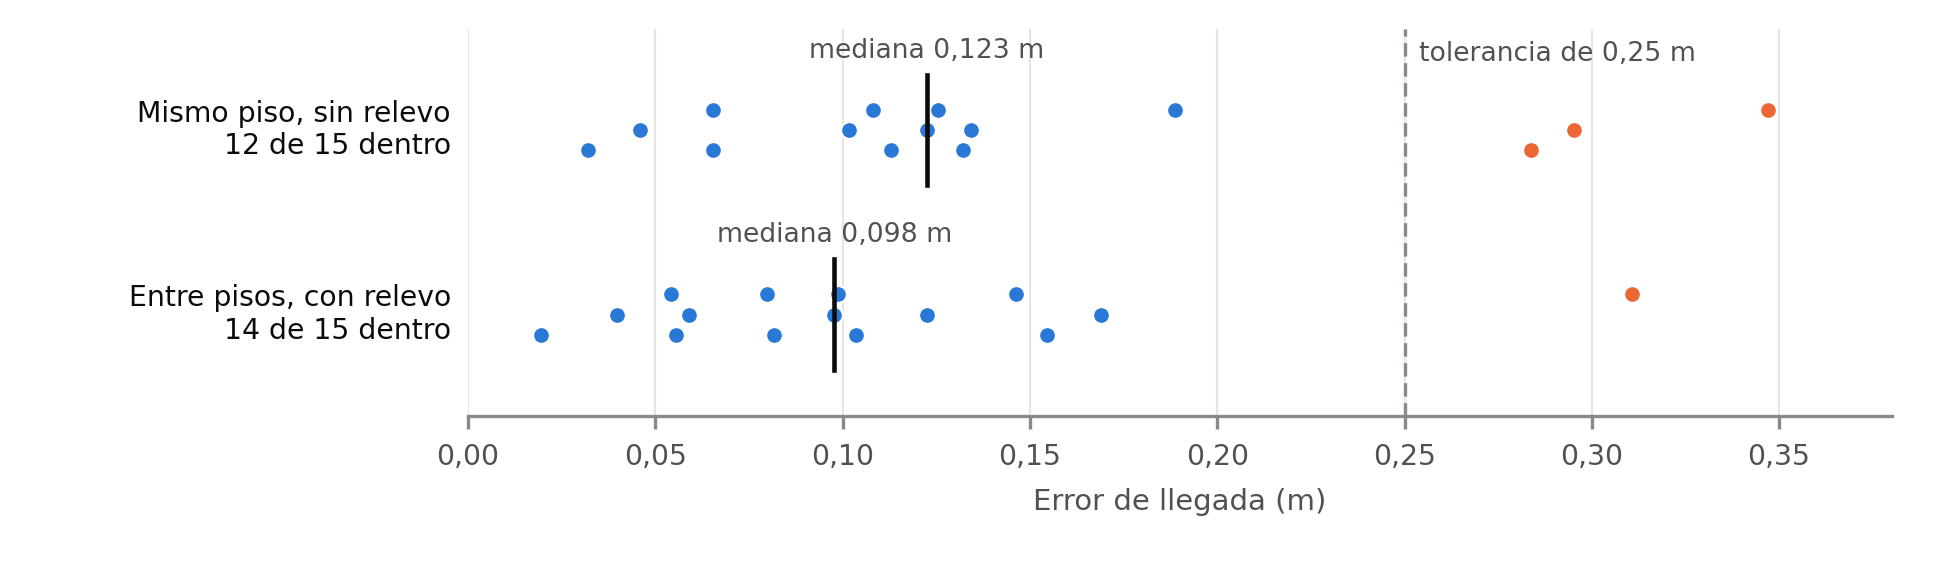
\includegraphics[width=\textwidth]{imagenes/llegada_simulacion.png}
  \caption{Error de llegada de las treinta misiones de la campaña en simulación, por grupo. La línea discontinua es la tolerancia de 0,25~m; en naranja, las cuatro misiones que quedaron fuera de ella. La marca vertical de cada fila es su mediana.}
  \label{fig:llegada-sim}
\end{figure}

\subsection{Tiempo de respuesta y tiempo de asignación}

El tiempo de respuesta se presenta por escalones, sin media ni desviación, debido a una limitación del instrumento (tabla~\ref{tab:respuesta}).

\begin{table}[htbp]
  \caption{Tiempo de respuesta de las treinta misiones, en escalones del reloj de
    la simulación.}
  \label{tab:respuesta}
  \begin{tabular}{@{}lcccc@{}}
    \toprule
    \textbf{Tiempo de respuesta} & 0,1 s & 0,2 s & 0,3 s & 0,4 s \\ \midrule
    Misiones & 10 & 15 & 4 & 1 \\ \bottomrule
  \end{tabular}
\end{table}

Los cuatro valores son múltiplos exactos de 100~ms, el paso con que avanza el reloj de la simulación, y la resolución del instrumento vale entre el 25~\% y el 100~\% de la magnitud medida. Una mediana de 0,2~s significa «uno o dos pasos del reloj», no «doscientos milisegundos», de manera que dar media y desviación sugeriría una precisión que el reloj no entrega. La cota, en cambio, sí se sostiene, y además es lo que le importa a un usuario: el agente arranca en menos de medio segundo.

El tiempo de asignación quedó por debajo de 100~ms en las treinta misiones, varios órdenes de magnitud por debajo de un paso del reloj, razón por la cual se caracterizó aparte, en un banco de pruebas con el reloj del sistema: mediana entre 154 y 175~\textmu s y máximo de 306~\textmu s. La figura~\ref{fig:simulacion} muestra una misión de la campaña.

\begin{figure}[htbp]
  \centering
  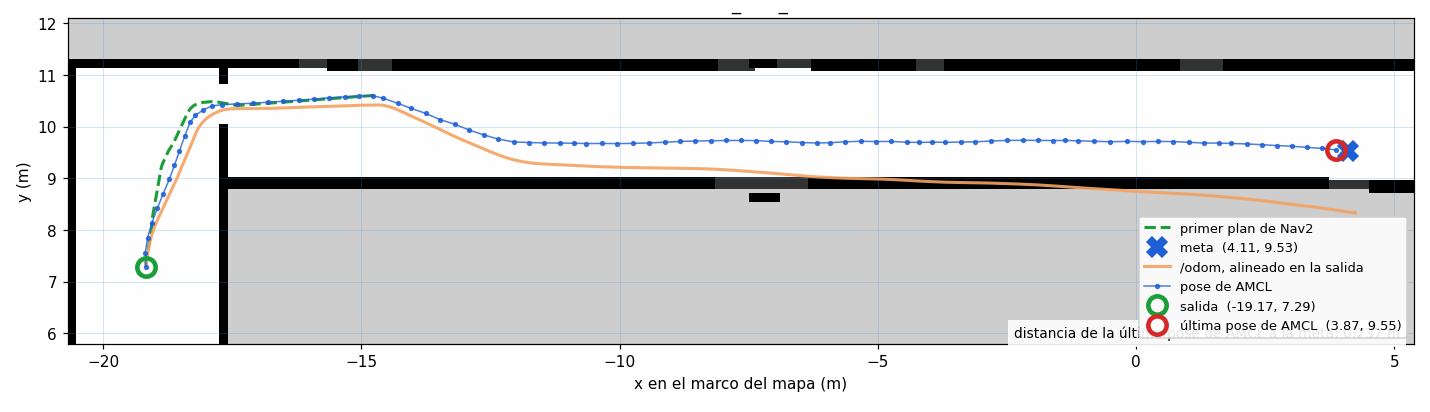
\includegraphics[width=\textwidth]{imagenes/corrida_simulacion.png}
  \caption{Una misión de la campaña en simulación. Se superponen el primer plan
    que calcula el navegador, la pose estimada a lo largo del recorrido y la
    odometría cruda. La separación creciente entre las dos últimas es la deriva
    que la localización corrige contra el mapa.}
  \label{fig:simulacion}
\end{figure}

% ---------------------------------------------------------------------
\section{Evaluación con los agentes físicos}
\label{sec:res-hw}

\subsection{La odometría del agente}

La odometría del agente sale de comparar barridos sucesivos del láser, y entre el 26 de agosto y el 2 de octubre no produjo una medida utilizable. La tabla~\ref{tab:odometria}
reúne lo que se midió en cada entorno, como fracción del avance real medido con
flexómetro.

\begin{table}[H]
  \centering\small
  \caption{Fracción del avance real que registra la odometría, por entorno. El
    criterio de la prueba es un error de 10~\% o menos.}
  \label{tab:odometria}
  \begin{tabular}{@{}p{0.44\textwidth}ccl@{}}
    \toprule
    \textbf{Entorno} & \textbf{Recorrido} & \textbf{Registrado} & \textbf{Criterio} \\ \midrule
    Gregorio, pasillo simulado (46,9 m de extensión en su mapa) & largo & 37,9 \% & no cumple \\
    Gregorio, pasillos simulados de los pisos 2 y 3 & largo & 5,7 \% y 1,3 \% & no cumple \\
    Gregorio, hall del piso 3 & 6 m & 73 \% & no cumple \\
    Cuarto cerrado, desplazado a mano & 3 m & 96,3 -- 101,9 \% & cumple \\
    Catalayud, pasillo del piso 4 & 6,68 m & 95,4 \% & cumple \\
    Catalayud, pasillo del piso 4 & 14,57 m & 103,3 \% & cumple \\
    Catalayud, piso 4, con la unidad inercial & 8,08 m & 101,9 \% & cumple \\
    Catalayud, piso 4, con la unidad inercial & 2,82 m & 104,9 \% & cumple \\ \bottomrule
  \end{tabular}
\end{table}

El estimador es el mismo en todas las filas: lo que cambió fue el entorno. En un pasillo con hornacinas, casilleros y quiebres, con ocho cambios de perfil en 25~m, la odometría queda dentro del $\pm$5~\% sin cambiar un parámetro. Con las dos mediciones del pasillo del piso 4, de 6,68 y 14,57~m, cumplió el criterio de la prueba, del que dependía todo lo demás con los agentes físicos. Las dos últimas filas ya incluyen la unidad inercial; el segundo de esos tramos mide 2,82~m, por debajo de los 5~m que pide el criterio, y se incluye como dato de la misma cadena.

\subsection{La navegación y la precisión de llegada}
\label{sec:res-g3}

La prueba de navegación de un agente pide un recorrido de punto a punto con Nav2 y la llegada verificada con flexómetro, a 0,5~m o menos del destino. En la primera sesión en el piso 4, el 2 de octubre, las dos llegadas medidas quedaron a 0,57 y 0,62~m, cortas, debido a que Nav2 daba entonces la meta por alcanzada a 1,0~m. Con la unidad inercial integrada, ese margen bajó a 0,5~m. El 7 de octubre, uno de los agentes recorrió en el piso 4 tres tramos encadenados, sin que nadie lo tocara entre uno y otro, y después regresó a la salida (tabla~\ref{tab:g3} y figura~\ref{fig:cadena}).

\begin{table}[htbp]
  \centering\small
  \caption{Cadena de tres tramos en el piso 4 y regreso a la salida: llegada de
    cada tramo.}
  \label{tab:g3}
  \begin{tabular}{@{}llcccl@{}}
    \toprule
    \textbf{Tramo} & \textbf{Destino} & \textbf{Tiempo} & \textbf{Recuperaciones} & \textbf{A la meta} & \textbf{Medida} \\ \midrule
    1 & Salón 403 & 13,5 s & 1 & 0,26 m & estimada \\
    2 & Salón 402 & 27,8 s & 1 & 0,45 m & flexómetro \\
    3 & Salón 401 & 5,2 s & 0 & 0,06 m & flexómetro \\
    Regreso & Salida & 62,8 s & 6 & 0,34 m & flexómetro \\ \bottomrule
  \end{tabular}
\end{table}

Las llegadas medidas quedaron dentro de la tolerancia de 0,5~m, y la prueba se superó. La llegada al Salón 403 no se midió porque en ese momento no había flexómetro, y se estimó con el error de los otros dos tramos. El regreso a la salida incluyó una media vuelta en el tramo ancho frente a los salones, que Nav2 resolvió con seis recuperaciones.

\begin{figure}[htbp]
  \centering
  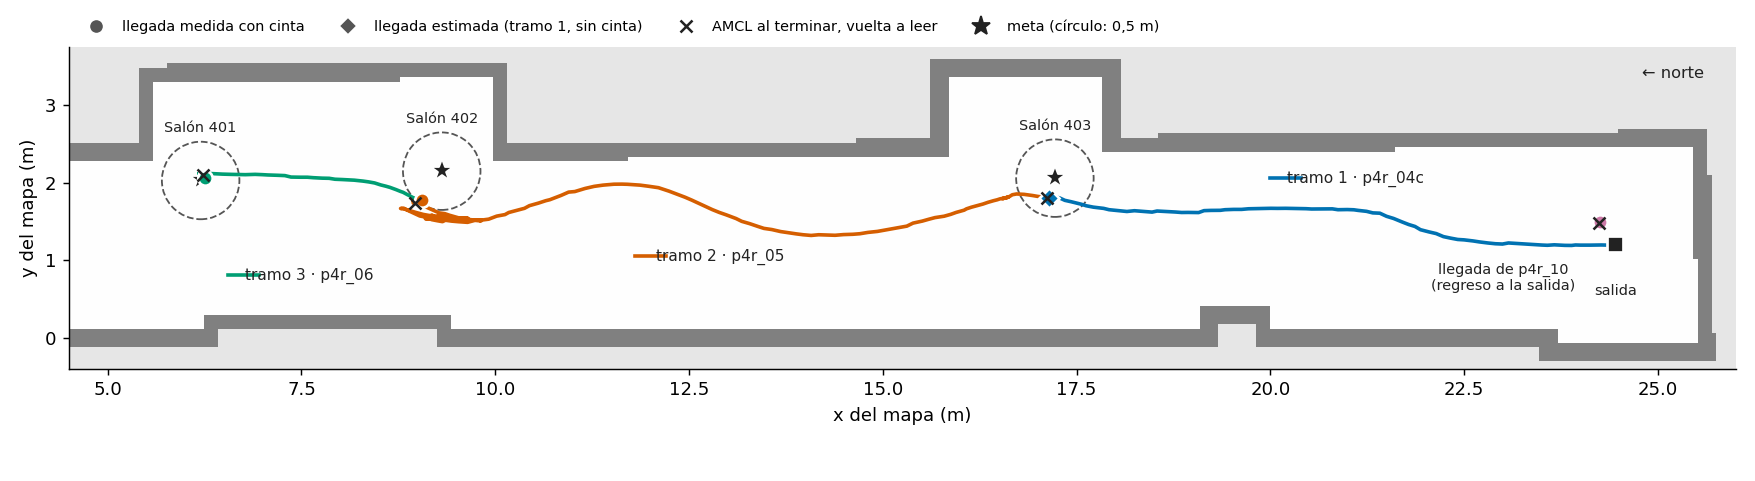
\includegraphics[width=\textwidth]{imagenes/cadena_piso4.png}
  \caption{Cadena de tres tramos en el piso 4 y regreso a la salida: recorrido
    según la localización, llegadas medidas con flexómetro, la llegada estimada
    al Salón 403 y la pose de la localización al terminar cada tramo.}
  \label{fig:cadena}
\end{figure}

El 8 de octubre, el otro agente recorrió el piso 3 en cinco tramos encadenados, con dos medias vueltas entre ellos, y los cinco terminaron con éxito y sin recuperaciones. Esas llegadas no se midieron con flexómetro, y al forzar a la localización a recalcular su pose al final de cada tramo, esta se desplazó entre 0,61 y 0,86~m. La pose que publica la localización al detenerse el agente va atrasada, por lo que la llegada que vale es la medida con flexómetro. La precisión de llegada sigue condicionada por la banda muerta de tracción, ya que el agente se aproxima a la meta a 0,40~m/s y no tiene régimen de aproximación fina.

% ---------------------------------------------------------------------
\section{Evaluación del sistema completo con los agentes físicos}
\label{sec:res-completo}

El 16 de octubre, el sistema completo funcionó con los dos agentes físicos (anexo A, video 7). La misión con relevo del Salón 302 al Salón 402 se completó, y de las diez misiones sorteadas para la campaña, las nueve que llegaron a ejecutarse se completaron, todas con relevo. La décima quedó interrumpida porque el computador portátil se apagó por falta de batería.

\subsection{Condiciones de las pruebas}

Las pruebas se hicieron en los pisos 3 y 4 del edificio Catalayud, con un agente en cada piso. El coordinador y el grabador se ejecutaron en el portátil, y cada misión se pidió desde la página web en un teléfono conectado a la red de los agentes. Los autores hicieron de usuario: pidieron cada misión, acompañaron a los agentes y confirmaron el cambio de piso en la página. Los agentes no se reubicaron entre misiones, y cuando el destino quedaba detrás del agente, el coordinador pidió la media vuelta en varios tiempos. La llegada se verificó con la localización de cada agente, sin medida con flexómetro.

\subsection{La misión con relevo}

La primera prueba del sistema completo fue una misión del Salón 302, en el piso 3, al Salón 402, en el piso 4, que se completó en 132,5~s, con un relevo y con la llegada a 0,444~m del destino. Entre la llegada del primer agente a la escalera y el arranque del segundo pasaron 61,1~s. Fue el segundo intento: en el primero, el coordinador rechazó la llegada del agente del piso 3 al Salón 302, adonde iba a recoger al usuario, porque su localización lo situaba a 0,59~m del punto.

Esa sesión sirvió de ensayo del montaje, y en ella las misiones se eligieron sin seguir el sorteo, de modo que no forman parte de la campaña. De las doce misiones grabadas, siete se completaron y cinco terminaron fallidas: en cuatro, el coordinador rechazó una llegada con el agente a entre 0,51 y 0,78~m del punto, y en la otra Nav2 abortó la navegación.

\subsection{La campaña con las misiones sorteadas}

Las diez misiones de la campaña se sortearon antes de ejecutarlas, con una semilla fija, entre los puntos de interés de los dos pisos: cinco de subida y cinco de bajada. Se ejecutaron en el orden del sorteo, y la tabla~\ref{tab:campana-vehiculos} da el resultado de las nueve que llegaron a ejecutarse.

\begin{table}[htbp]
  \centering\small
  \caption{Campaña con los agentes físicos: las nueve misiones sorteadas que se
    ejecutaron, todas completadas con un relevo. La llegada es la de la
    localización del agente, con una tolerancia de 0,5~m.}
  \label{tab:campana-vehiculos}
  \begin{tabular}{@{}cllccc@{}}
    \toprule
    \textbf{N.\textsuperscript{o}} & \textbf{Origen} & \textbf{Destino} & \textbf{Tiempo total} & \textbf{Respuesta} & \textbf{Llegada} \\ \midrule
    1 & Ascensor, piso 3 & Salón 403 & 52,3 s & 0,51 s & 0,435 m \\
    2 & Salón 302 & Salón 401 & 90,1 s & 0,27 s & 0,202 m \\
    3 & Salón 401 & Salón 302 & 87,6 s & 3,90 s & 0,143 m \\
    4 & Salón 403 & Salón 303 & 78,9 s & 1,25 s & 0,420 m \\
    5 & Salón 402 & Salón 301 & 105,4 s & 0,66 s & 0,285 m \\
    6 & Salón 301 & Salón 401 & 89,8 s & 2,97 s & 0,226 m \\
    7 & Ascensor, piso 4 & Salón 301 & 81,7 s & 0,87 s & 0,234 m \\
    8 & Salón 302 & Salón 403 & 81,8 s & 0,95 s & 0,214 m \\
    9 & Salón 303 & Salón 402 & 92,6 s & 0,63 s & 0,299 m \\ \midrule
    \multicolumn{3}{@{}l}{Mediana} & 87,6 s & 0,87 s & 0,234 m \\ \bottomrule
  \end{tabular}
\end{table}

Con nueve éxitos en nueve misiones, el intervalo de Wilson al 95~\% va del 70,1 al 100~\%, lo que permite afirmar que la tasa de éxito con los agentes físicos supera el 70~\%, la misma cota que sostiene la campaña en simulación. Con la expresión de la norma ASTM F3244-21, nueve repeticiones sin fallo demuestran una fiabilidad mínima de 0,81 con un 85~\% de confianza.

El error de llegada tuvo una mediana de 0,234~m y fue de 0,143 a 0,435~m. El tiempo total, desde la solicitud hasta la llegada verificada, tuvo una mediana de 87,6~s y fue de 52,3 a 105,4~s. El tiempo de respuesta, desde que el coordinador acepta la solicitud hasta que el agente asignado empieza a moverse, tuvo una mediana de 0,87~s y quedó por debajo de 1,3~s en siete de las nueve misiones. Los dos valores más altos, 3,90 y 2,97~s, son de misiones en que el agente ya estaba en el punto de origen: el coordinador verificó esa llegada, que no exigía moverse, con la espera de 1,5~s, y el primer movimiento fue la media vuelta hacia la escalera. El tiempo de asignación fue de 0,3~ms en las nueve misiones, medido con el reloj del portátil e incluyendo el paso del mensaje hasta el grabador, del mismo orden que el del banco de pruebas. En las nueve misiones los agentes hicieron 24 medias vueltas, de entre 160 y 171$^\circ$, en uno a cuatro tiempos cada una.

La figura~\ref{fig:campana-vehiculos} descompone el tiempo de cada misión en sus etapas. Ir a recoger al usuario tomó entre 2,2 y 30,6~s, según dónde había terminado la misión anterior, mientras que el guiado en el piso de origen tuvo una mediana de 24,2~s, y el guiado en el piso de destino, de 24,8~s.

\begin{figure}[htbp]
  \centering
  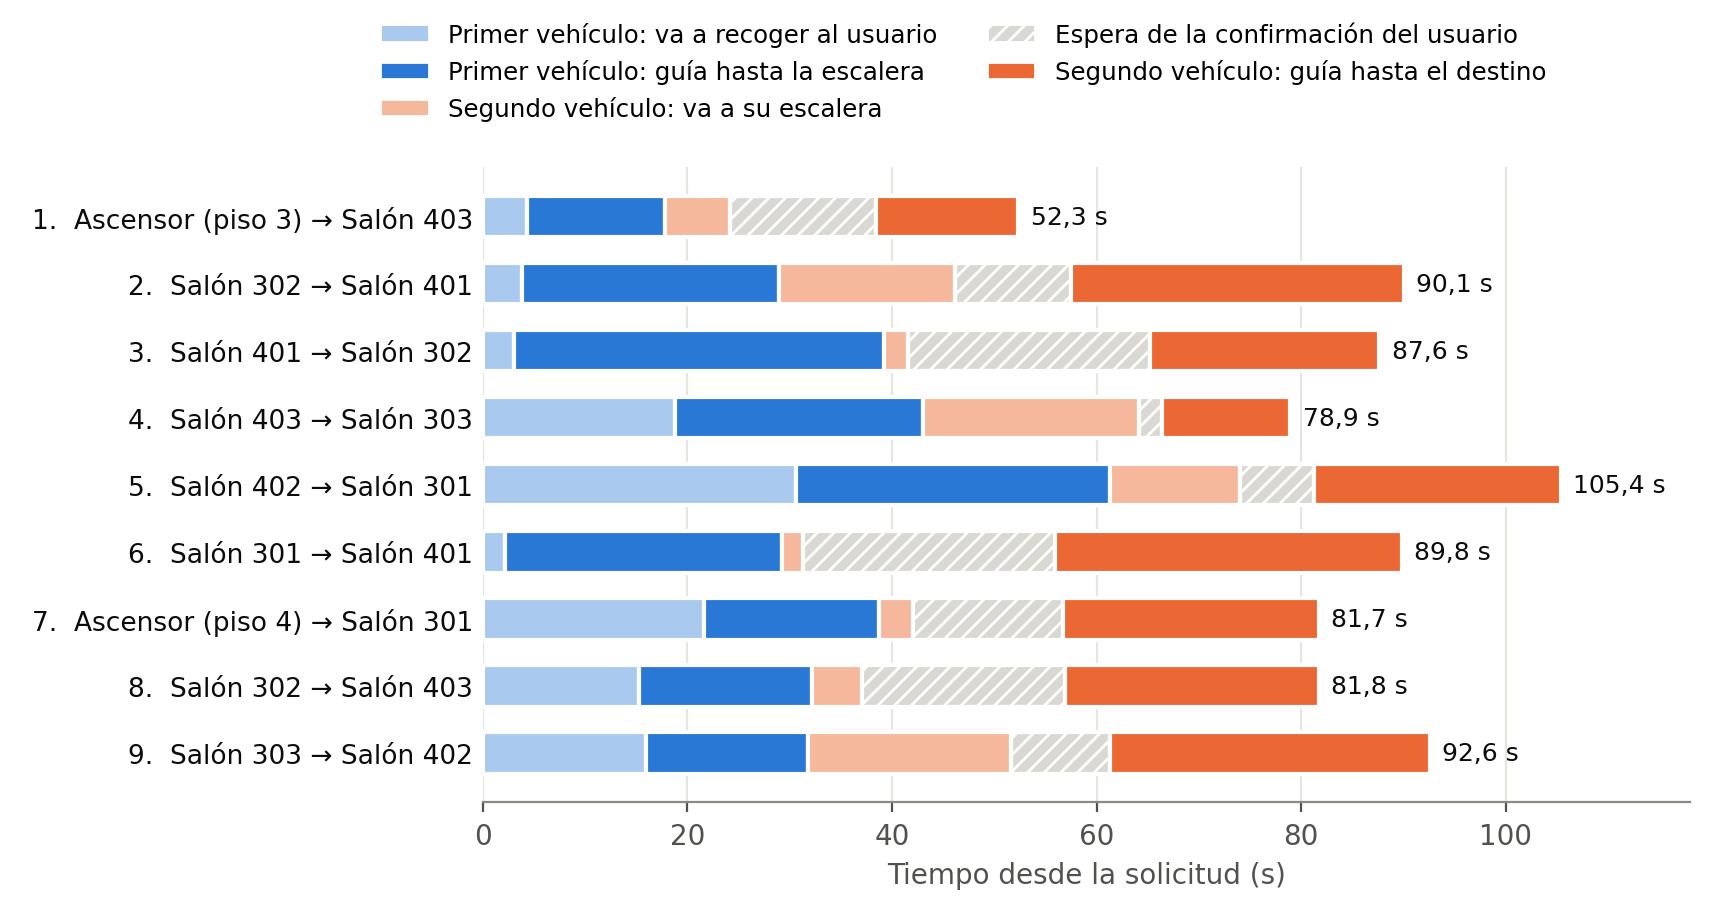
\includegraphics[width=\textwidth]{imagenes/campana_vehiculos_etapas.png}
  \caption{Duración de cada etapa en las nueve misiones de la campaña con los agentes físicos, según las marcas de etapa del coordinador. El tramo rayado es la
    espera de la confirmación de cambio de piso, contada desde que el segundo
    agente está en su escalera.}
  \label{fig:campana-vehiculos}
\end{figure}

\subsection{El relevo entre los dos agentes}

En las nueve misiones el relevo se produjo y el coordinador no pasó por el estado inactivo ni quedó sin agente asignado, aunque, como en simulación, ese criterio no puede fallar por la forma en que está construido. La medida que informa es el intervalo del relevo: el tiempo desde que el primer agente llega a su escalera hasta el primer movimiento del segundo.

Ese intervalo tuvo una mediana de 1,22~s, pero la cifra junta dos situaciones. En cinco misiones el segundo agente tuvo que desplazarse hasta su escalera, en cuatro desde el destino de la misión anterior y en una para corregir su posición, y arrancó en menos de 1,3~s. En las otras cuatro ya estaba en la escalera, su primer movimiento fue el del guiado final, después de la confirmación, y el intervalo, de 12,9 a 27,5~s, mide sobre todo cuánto tardó el usuario en confirmar.

Para el usuario, el tiempo que importa es el que pasa entre la llegada a la escalera del piso de origen y el arranque del guiado en el piso de destino, durante el cual cambia de piso, el segundo agente llega a su escalera si no estaba allí, y el usuario confirma en la página. Ese tiempo tuvo una mediana de 24,8~s y fue de 18,0 a 29,5~s. La confirmación, desde que el segundo agente estaba en su escalera, tomó entre 2,3 y 24,7~s, y el aviso de los 60~s no llegó a mostrarse en ninguna misión.

\subsection{Criterio de conteo e incidencias}

En la tasa de éxito cada misión cuenta una sola vez, con el intento que se completó, mientras que el protocolo cuenta como fallo toda ejecución fallida. Por esa razón conviene declarar los intentos que la tasa deja fuera. Después de reiniciar las cadenas de navegación, las misiones 1 y 2 se completaron al segundo intento. Los dos intentos fallidos ocurrieron en el tramo en que el agente del piso 3 iba a recoger al usuario: en el de la misión 1, el coordinador rechazó la llegada al ascensor, con el agente a 0,526~m del punto, y en el de la misión 2 no tenía la pose del agente para verificar la llegada. En los dos casos el coordinador actuó como estaba previsto, y lo que faltó fue la precisión o la pose del agente.

Antes de esos intentos, la navegación de los dos agentes dejó de responder, y ocho intentos de la misión 1 terminaron rechazados o abortados, con las transformadas de posición detenidas dentro de Nav2. La detención ocurrió después de que el portátil se apagara por falta de batería, con los agentes ya con horas encendidos y con cargas de 10 a 14 en procesadores de dos núcleos. Se reiniciaron las cadenas de navegación con la pose de salida, y después las nueve misiones se ejecutaron sin tocar los agentes.

La misión 10 empezó y no terminó, pues el portátil volvió a apagarse por falta de batería poco después de pedirla, cuando el agente del piso 4 ya había llegado a su escalera. Antes se había pedido por error el ascensor del piso 4 como destino, debido a que los ascensores de los dos pisos aparecían en la página con el mismo nombre; ese intento no es una misión del sorteo y no se cuenta. Después de la campaña, la página muestra el piso junto a los nombres que se repiten.

% ---------------------------------------------------------------------
\section{Limitaciones de la medición}
\label{sec:limitaciones}

\subsection{Naturaleza del criterio de continuidad entre niveles}

La continuidad del servicio es la variable de respuesta principal del cuarto objetivo, y su criterio binario se cumplió en las treinta misiones. Ese resultado, sin embargo, no es evidencia: el criterio exige que, dentro de la ventana de la misión, el coordinador nunca esté inactivo ni tenga el agente sin asignar, y los dos únicos puntos del código que producen esos valores ocurren antes de que la ventana se abra. Como no existe ejecución posible que lo incumpla, el criterio no puede dar un resultado negativo y no aporta evidencia, por muchas veces que se verifique.

No se corrigió inventando una ruta de fallo, ya que eso habría sido instrumentar el experimento para que pareciera más informativo. La continuidad se declaró como un invariante estructural del diseño, y la afirmación se apoyó en una magnitud que sí varía: el intervalo del relevo, entre el final del tramo de un agente y el inicio del tramo del otro. En las quince misiones entre pisos tuvo una mediana de 0,1~s y un máximo de 0,2~s, es decir, uno o dos pasos del reloj de la simulación.

\subsection{Espacio desconocido marcado como libre en el mapa}

El mapa de ocupación es una imagen en la que cada celda es libre, ocupada o desconocida, y su archivo de configuración fija el umbral por debajo del cual una celda se carga como libre. En el mapa de la campaña en simulación ese umbral era 0,25, y las celdas desconocidas, que el formato guarda con una ocupación de 0,196, quedaban por debajo de él. Al cargar el mapa, 10\,908 celdas que el modelo no describía, el 14,5~\% del mapa, se leyeron como espacio libre. Con eso, las dos protecciones que impiden planificar por espacio desconocido, la del planificador y la del mapa de costos, no tenían nada que rechazar.

El defecto no cambia el veredicto de la campaña, puesto que los cuatro fallos fueron de precisión de llegada, sin relación con el trazado, y el pasillo por el que se navegó es libre en el mundo simulado. Queda sin verificar que ninguna trayectoria cruzara una de esas celdas, algo que se puede comprobar con los registros conservados. El umbral se corrigió a 0,10 el 25 de septiembre, después de la campaña.

\subsection{La llegada en los agentes físicos, sin medida externa}
\label{sec:lim-llegada}

En la campaña con los agentes físicos la llegada no tuvo una medida independiente del sistema. El protocolo la toma con flexómetro sobre marcas en el piso, y en esa sesión no se midió, aunque la odometría y la llegada ya se habían verificado con flexómetro en los mismos pisos, en las pruebas de odometría y de navegación. El error que se informa es el de la localización del propio agente contra el punto del catálogo, leído 1,5~s después de que Nav2 diera la meta por alcanzada, con el agente ya detenido. Es la medida con que el coordinador acepta la llegada, así que el sistema verificó su llegada con su propia estimación, que es lo que la regla principal del protocolo procura evitar. Los registros lo declaran con la procedencia de la medida, y el programa de análisis lo advierte al calcular las métricas.

La única comparación entre la localización y el flexómetro en los agentes físicos es la de la cadena de tres tramos en el piso 4, donde la localización, leída de nuevo al terminar cada tramo, quedó a 0,10~m o menos de la medida en el sentido del avance y a 5~cm o menos de lado. En el piso 3, en cambio, forzar a la localización a recalcular su pose al final de cada tramo la desplazó entre 0,61 y 0,86~m. Por lo tanto, el resultado de la campaña se lee así: cada agente, según su propia localización, llegó a menos de 0,5~m del destino, y queda sin medir si la distancia real cumplió la misma tolerancia.
